\section{Artificial Neural Networks}\label{ANNsection}
Nonlinear methods for function approximation involve \textit{artificial neural networks} (ANNs). ANNs are the product of inspiration from the neural networks in the brains of animals and humans. Their properties and functionality have been successfully replicated in ANNs. An ANN is a layered structure of neurons which has minimum one input layer and one output layer. Each layer has a number of units (neurons) that are connected to the units in another layer. The connections are assigned weights that are used for the unit's \textit{activation}. In order to perform activation, a weighted sum of it's inputs is computed at each unit and then passed to an activation function to produce output. There are different activation functions, though, and the choice depends on the type of problem.

In dependence of the structure of the network, there are different types of ANNs. For example, a simple case of \textit{feedforward} ANN without any loops, with an input layer of 4 units, 2 hidden layers, and an output layer with 2 units is presented in the \Cref{fig:feedforward}:
\begin{figure}[H]
	\centering
	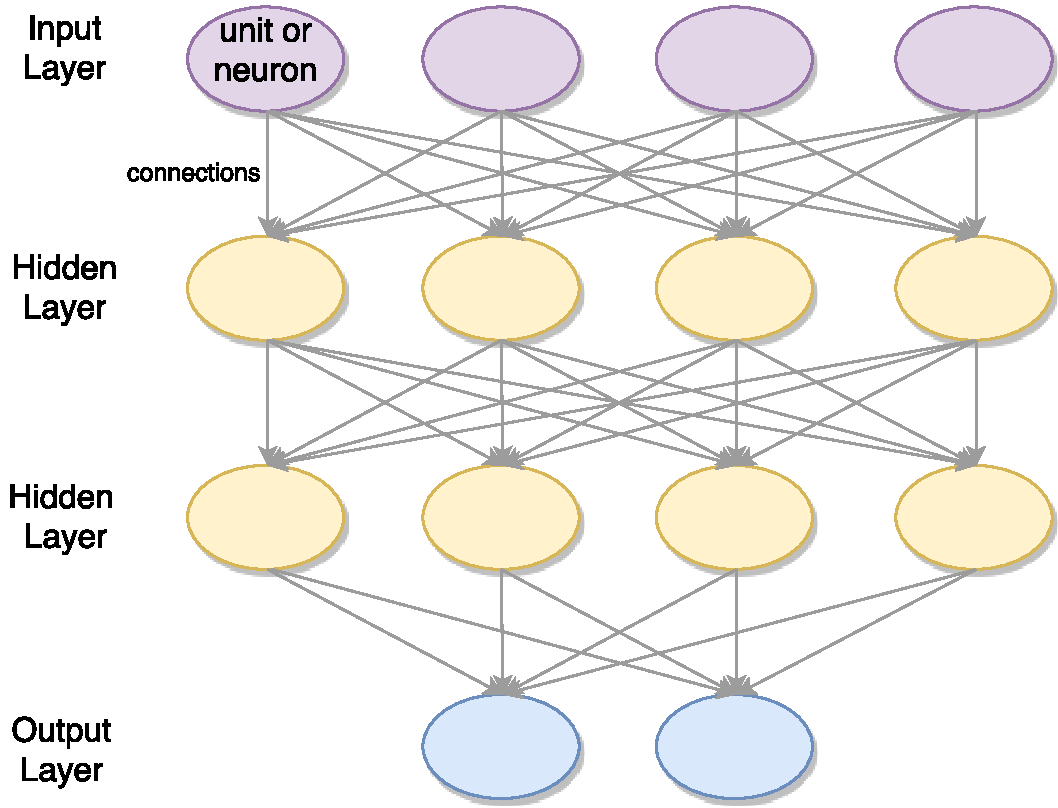
\includegraphics[width=0.7\textwidth]{Figures/Feedforward}
	\caption{Feedforward ANN}
	\label{fig:feedforward}
\end{figure}
Some ANNs can be called \textit{deep}. This qualifier describes the networks that have many hidden layers, precisely more than two. More hidden layers would compute more abstract representations of the input data, which means richer features. Deep ANNs are harder to train, but they are more powerful, and are especially used in modern artificial intelligence applications.

Usually, ANNs learn by a SGD method. More precisely, learning implies the definition of an objective function that describes the performance of the network, and, which is either minimized or maximized. An objective function can be the loss of the network over a set of training examples. In RL, an ANN can use TD errors in computing the loss function and learning the value function, or maximize the reward, or use a policy-gradient algorithm \cite{Sutton}. No matter the case, the partial derivatives are required to determine the influence of a weight change on the network's performance, and they can be obtained with the help of the gradient.

In order to find the gradient, an ANN can use the back-propagation algorithm. In the forward pass, the network's units would compute the outputs, whereas in the backward pass - the partial derivatives with respect to each weight. However, the back-propagation algorithm isn't that efficient for the deep ANNs, because of the overfitting problem.

A special structure of the network's architecture, like that of the deep \textit{convolutional networks} (CNN) would make it possible to use the back-propagation algorithm in deep ANNs, too. CNN is a very important type of ANN that is especially used for finding spatially correlated patterns in images while sharing weights and excluding the need of full connectivity between units.

\subsection{Convolutional Neural Networks (CNNs)} \label{subsectionCNN}

Convolutional Neural Networks are like normal neural networks. They are made up of neurons that can learn weights and biases. Each neuron receives some inputs, perform a dot product and sometimes follows it with a non-linearity. The whole network expresses a single differentiable score function - from raw image pixels to class scores. CNN architectures assume that the inputs are images, which make it possible to encode certain properties into the architecture. It makes the forward function more efficient to implement and reduce the number of parameters in the network. \cite{CNN_course}           

The problem about regular neural networks is it doesn't scale well to full images. An example is the CIFAR-10 \cite{CIFAR_10}, Here are the images only of size 32x32x3 (32 wide, 32 high, 3 color channels). A single fully-connected neuron in first hidden layer of a regular Neural Network would have $32\cdot32\cdot3 = 3072$ weights. For images in bigger sizes, e.g. 200x200x3, would lead to neurons that have $200\cdot200\cdot3 = 120,000$ weights. This full connectivity is wasteful and the huge number of parameters would quickly lead to overfitting.

Convolutional neural networks take advantages of the fact that the input consist of images. It is done by instead of in regular neural networks, the layers of a CNN have neurons arranged in 3 dimensions: width, height, depth. Example of the CIFAR-10 are an input volume of activations, and the volume has dimensions 32x32x3 (width, height, depth respectively). The neurons in a layer will only be connected to a small region of the layer before it, instead of all the neurons in a fully-connected manner. To see this different we compare \Cref{fig:feedforward} with the figure below \Cref{fig:NN_vs_CNN}.    

\begin{figure}[H]
	\centering
	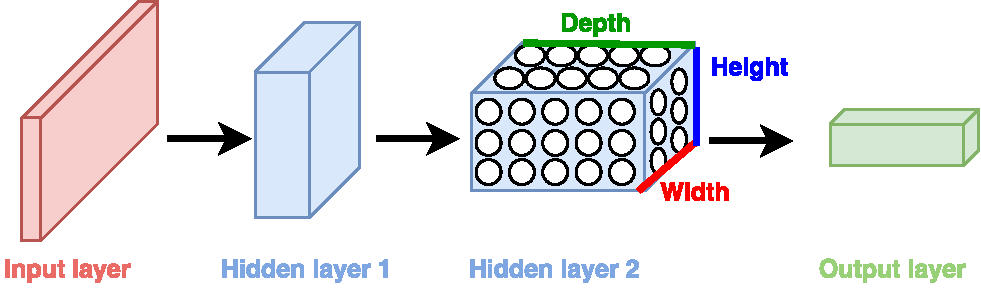
\includegraphics[width=1\textwidth]{Figures/NN_vs_CNN.pdf}
	\caption{A Convolutional Neural Network arranges its neurons in three dimensions (width, height, depth), as visualized in one of the layers. Every layer of a ConvNet transforms the 3D input volume to a 3D output volume of neuron activations. In this example, the red input layer holds the image, so its width and height would be the dimensions of the image, and the depth would be 3 (Red, Green, Blue channels) \cite{CNN_course}}
	\label{fig:NN_vs_CNN}
\end{figure}

\subsubsection{Layers}
As described earlier a CNN is a combination of layers and every layer transforms one volume of activations to another through a differentiable function. CNN uses three main types of layers to build the architecture: Convolutional Layer, Pooling Layer, and Fully-Connected Layer (exactly as seen in regular Neural Networks on \Cref{fig:feedforward}). We will stack these layers to form a full CNN architecture. In reinforcement learning is the pooling layer not used, because they buy translation invariance - the network becomes insensitive to the location of an object in the image.

\subsubsection{Convolutional Layer}
The Convolutional layer is the main building block of a convolutional neural network it does most of the computational heavy lifting. The convolutional layer consists of learnable filters. Every filter is small spatially (along width and height), but extend through the full depth of the input volume. An example of the first layer in a CNN is a filter with size 5x5x3. During the first forward pass, it is slide/convolved each filter across the height and width of the input volume and compute dot products between the entries of the filter and the input at any position. As the filter slide over the input volume it produces a 2-dimensional activation map. The activation map shows the responses of that filter at all spatial positions. The network will learn filters that activate when they see some type of visual feature - such as an edge of some orientation or a patch of some colors. On higher layers the network will learn to see more advance patterns, it could be honeycomb or wheel-like patterns. On each convolutional layer, it will have an entire set of filters, each layer will produce a separate 2-dimensional activation map. The activation maps will be stacked along the depth dimension and produce the output volume. 

When dealing with high dimensional inputs like images, it is impractical to connect neurons to all neurons in the previous volume. Instead it is smart to connect each neuron to only a local region of the input volume. The spatial extent of this connectivity is a hyperparameter called the receptive field of the neuron - equivalently this is the filter size. An illustration of the receptive can be seen on \Cref{fig:Respective_field}

\begin{figure}[H]
	\centering
	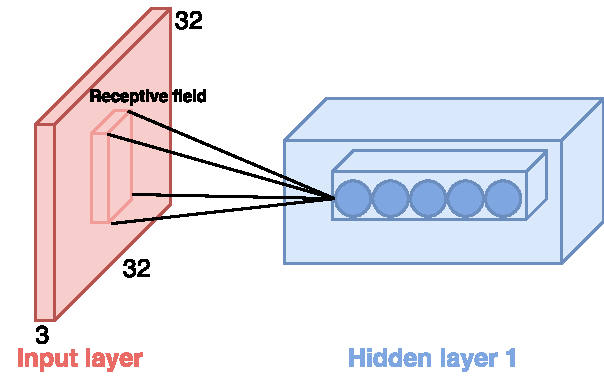
\includegraphics[width=0.7\textwidth]{Figures/Respective_field.pdf}
	\caption{An example input volume in red (e.g. a 32x32x3 CIFAR-10 image), and an example volume of neurons in the first Convolutional layer in blue. Each neuron in the convolutional layer is connected only to a local region in the input volume spatially, but to the full depth (i.e. all color channels). Note, there are multiple neurons (5 in this example) along the depth, all looking at the same region in the input \cite{CNN_course}}
	\label{fig:Respective_field}
\end{figure}

\textbf{Spatial arrangement}
The connectivity of each neuron in the convolutional layer to the input volume, is described by the spatial arrangement. Spatial arrangement includes how many neurons there are in the output volume and how they are arranged. Three hyperparameters control the size of the output volume - the depth, stride and zero-padding.. 

The first hyperparameter is the depth, it corresponds to how many filters the convolutional layer use. Each filter looking for something different in the input. An example is the convolutional layer takes a raw image as an input, then different neurons along the depth dimension may activate in presence of various oriented edges or blobs of colors. A set of neurons that are all looking at the same region of the input is called \textit{depth column} or \textit{fibre}

Another hyperparameter is the stride - it defines the stride the filters are slide over the input. If the stride is 1 the filters move one pixel at a time. When the stride is 2 then the filters moves 2 pixels at a time. This will produce smaller output volumes spatially.

The last hyperparameter to control the size of the output volume is the size of zero-padding. Zero-padding, pad the input volume with zeros around the border. The good feature with zero-padding is it control the spatial size of the output volumes. This is useful to preserve the spatial size of the input volume so the input and output width and height are the same. 

The way to compute the spatial size of the output volume as a function of the input volume size ($\textbf{W}$), the receptive field size of the convolutional layer neurons($\textbf{F}$), the stride with which they are applied ($\textbf{S}$) and the amount of zero padding used ($\textbf{P}$) on the border. The formula for calculating, how many neurons "fit" is:
\begin{equation}
\frac{W-F+2P}{S}+1
\end{equation}    
An example for a 5x5 input and a 3x3 filter with stride 1 and zero-padding 1 the output would be of the spatial size 5x5:
\begin{equation}
\frac{5-3+2\cdot1 }{1}+1         \rightarrow             \frac{4}{1}+1 =5
\end{equation} 
And with stride 2 the output would be 3x3:
\begin{equation}
\frac{7-3+2\cdot1 }{2}+1         \rightarrow             \frac{4}{2}+1 =3
\end{equation} 
The visualization can be seen on the figure below \Cref{fig:Spatial_size}: 

\begin{figure}[H]
	\centering
	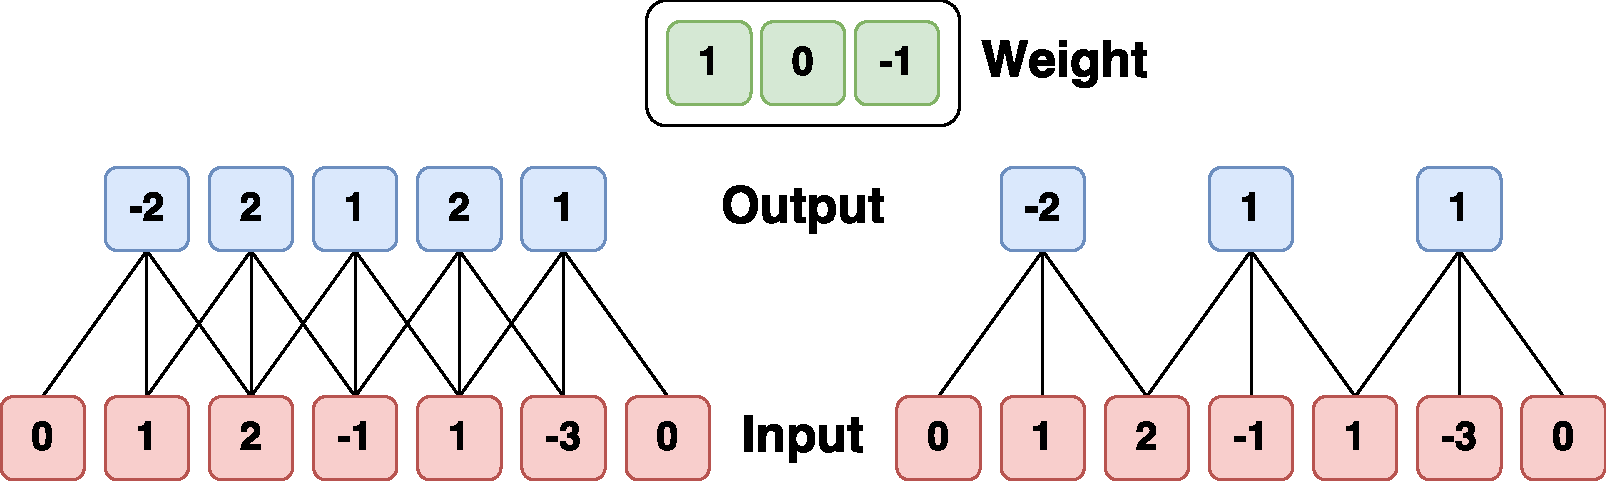
\includegraphics[width=1\textwidth]{Figures/Spatial_size.pdf}
	\caption{Illustration of spatial arrangement. The example is described above. In this example, there is only one spatial dimension (x-axis), one neuron with a receptive field size of F = 3, the input size is W = 5, and there is zero padding of P = 1. \textbf{Left:} The neuron strided across the input in stride of S = 1. \textbf{Right:} The neuron uses stride of S = 2
	The neuron weights are in this example [1,0,-1] (shown on very right), and its bias is zero. These weights are shared across all yellow neurons. \cite{CNN_course}
	}
	\label{fig:Spatial_size}
\end{figure} 

\subsubsection{Summary of convolutional layers}
To summarize the convolutional layer
\begin{itemize}
	\item Accept a input volume of size $W_1 \times  H_1 \times  D_1$
	\item Requires four hyperparameters:
	\begin{itemize}
		\item Number of filters $K$
		\item The receptive field size of the Convolutional Layer neurons $F$ 
		\item The stride $S$
		\item The amount of zero-padding $P$ 
	\end{itemize}
	\item Output a volume of size $W_2 \times  H_2 \times  D_2$
	\begin{itemize}
		\item $W_2 = \frac{W_1-F+2P}{S}+1$
		\item $H_2 = \frac{H_1-F+2P}{S}+1$
		\item $D_2 = K$
	\end{itemize}
	\item In the output volume the $d$-th depth slide (of side $W_2 \times  H_2$) is the result of performing a valid convolution of the $d$-th filter over the input volume with a stride of $S$, and then offset by $d$-th bias
\end{itemize}

\subsubsection{Fully connected Layer}
The fully connected layer is a traditional Multi-Layer Perceptron. The term “Fully Connected” implies that every neuron in the previous layer is connected to every neuron on the next layer as seen on \Cref{fig:feedforward}. The output from the convolutional layers represent a high-level feature of the input image. The purpose of the Fully Connected layer is to use these features for classifying the input image into various classes. 

Apart from classification fully connected layer is also a cheap way to learn non-linear features from these layers. By combining these features, the classification of the network would be even better \cite{Fully_Connected_Layer}.
.

\subsection{Recurrent Neural Networks (RNNs)} \label{RNN}
Recurrent neural networks (RNN) are used when the patterns in data change with time. RNNs have a simple structure with a built-in feedback loop allowing it to act as a forecasting engine. RNNs are applied in a large range of applications, from speech recognition to driver-less cars. Unlike feedforward neural networks where the data flows in one direction only, while in RNN the output of the layer is added to the input of the same layer, which represents the whole network. This results in a loop like network. The flow can be viewed or interpreted as a time passage where at each time-step the same layer receives it's own output from the previous time-step and adds it up to the input part together with the new data received \cite{RNNvideo}. 

Unlike feedforward ANNs, RNNs can work with sequences of data inputs and, subsequently, to output sequences of data in return. Not only RNNs use sequence of data, but also these sequences can vary in their size, so different sizes of sequences can be adapted by the RNN dynamically. Another key feature of the RNN is the dependency of the training examples. Unlike feedforward ANNs, where the training examples are independent of each other, the RNNs treat temporal dependencies, meaning that a sequence of e.g. words is usually dependent on what came before \cite{NeonRNN}. These new features open a new range of applications like image captioning (single input, sequence output), document classification (sequence input, single output), video frames classification (sequence input, sequence output), demand and supply chain planning forecasting (with added time delay) \cite{RNNvideo}.

In order to understand better the recurrent neuron functionality, the Figure \ref{Units} presents a comparison between the RNN unit and the linear unit used in feedforward ANNs.

\begin{figure}[H]
	\centering
	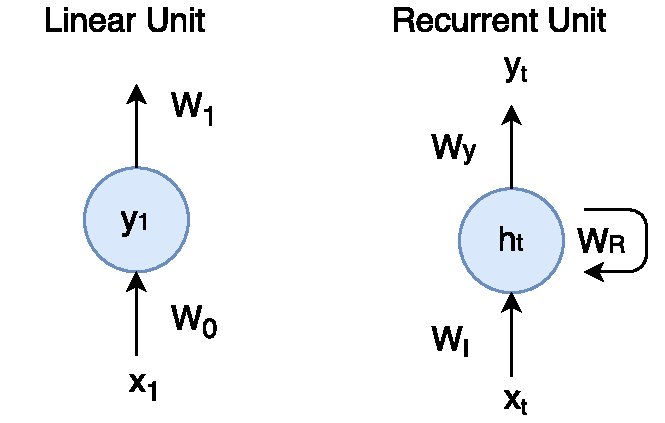
\includegraphics[width=0.5\textwidth]{Figures/RecurrentUnit}
	\caption{Linear vs. Recurrent unit}
	\label{Units}
\end{figure}
A linear unit's output is the input $x_{j}$ times the weight matrix $W_{ij}$ which is then passed to an activation function $g$.
\begin{equation}\label{linearOutput}
y_{i}=g(\sum_{j}W_{ij}x_{j}+b)
\end{equation}

The recurrent unit is composed of a linear unit, but then it adds a recurrent weight $W_{R}$, therefore the output $h^{(t)}$ depends on both the input $x_{t}$ and the activity at the previous time-step. To retrieve an output $y_{t}$ from the layer, a non linear activation function $g_{y}$ is applied to the $h^{(t)}$ \cite{NeonRNN}.
\begin{equation}\label{recurrentOutput}
\begin{aligned}
h^{(t)}&=g_{h}(W_{I}x^{(t)}+W_{R}h^{(t-1)}+b_{h})\\
y^{(t)}&=g_{y}(W_{y}h^{(t)}+b_{y})
\end{aligned}
\end{equation}

For example, in case of word prediction, the input of a unit can be a word, and the output of that unit would be the predicted next word that follows the one that was input; then, when the next input comes in at the next time-step, the process is applied, but also with the activity at the previous time-step taken into account.

The training of RNNs is different than that of the other ANNs, because RNNs emit an output at each time-step, and, therefore, there is a cost function at each time-step, whereas before, in feedforward networks, it was necessary to run the input through the whole network in order to get an output comparable to the one and only cost function. Another special characteristic of the RNNs is that the weights $W_{R}$ are shared across the network. So, the gradients from all the time-steps can be combined together to obtain the weights update and do back-propagation. But, because of the shared weights the update would scale with the size of the $W_{R}$, the back-propagation has to be done all the way until time-step zero, which causes the problem of vanishing and exploding gradients \cite{NeonRNN}.

In order to address the problems of training deep RNNs there are different solutions available. Among the known solutions are the use of the \textit{Root Mean Square Propagation} (RMSProp) optimizer for learning rate adjustment, clipping gradients, ReLu activation functions, special weight initialization, or to use \textit{gating} \cite{NeonRNN}. Gating is a technique for deciding when to forget the current input, and when to remember it for future time steps \cite{RNNvideo}. The most famous approaches are \textit{long short-term memory} (LSTM) and \textit{gated recurrent units} (GRU).

LSTM has at it's core a memory cell $C$ with a recurrent weight $W_{C}=1$ that inherits the activity of the previous time-step. This memory cell has three manipulations: \textit{forget} (flush the memory), \textit{input} (add to the memory), and \textit{output} (retrieve from the memory) \cite{NeonRNN}. The activity of the memory cell $C_{t}$ is taken and passed through a tanh activation function and multiplied by the \textit{gate}. The gate is an affine layer, or a 'standard' feedforward ANN layer, that has as inputs $x_{t}$ at the current time-step and $h_{t-1}$ of the previous time-step that are together multiplied by the weight $W_{0}$, summed and passed through the sigmoid activation function $\sigma$ to return a vector of numbers between $0$ and $1$. The gate operation for generating the \textit{output} $h_{t}$, or for getting the information from the memory cell $C_{t}$, is presented in the following equation:
\begin{equation}\label{gate}
\begin{split}
h_{t}&=\sigma(W_{0}\cdot \left [ x_{t} h_{t-1} \right ]+b_{0})\odot \textup{tanh}(C_{t})\\
&=o_{t}\odot \textup{tanh}(C_{t})
\end{split}
\end{equation}

The same approach is used for the \textit{forget} operation $f_{t}$. A layer before the final output is introduced, but with different weights, $W_{f}$. If the output of the forget gate is $0$, means that the memory has been flushed completely, whereas if the output is all $1$s then the memory retained everything \cite{NeonRNN}. The \textit{input} for the next time-step has two affine layers, one for generating new input $\widetilde{C_{t}}$ for the memory cell with the weights $W_{C}$ and tanh activation function, and another one $i_{t}$ that modulates the input and writes it into the memory cell with the weights $W_{i}$ and the sigmoid $\sigma$ activation function. All the components of the LSTM structure are vectors with numbers between $0$ and $1$, and they can be handled to perform either of the available manipulations. The summarized presentation of the LSTM components with the corresponding affine layers is illustrated in the Figure \ref{LSTMcore} \cite{NeonRNN}.
\begin{figure}[H]
	\centering
	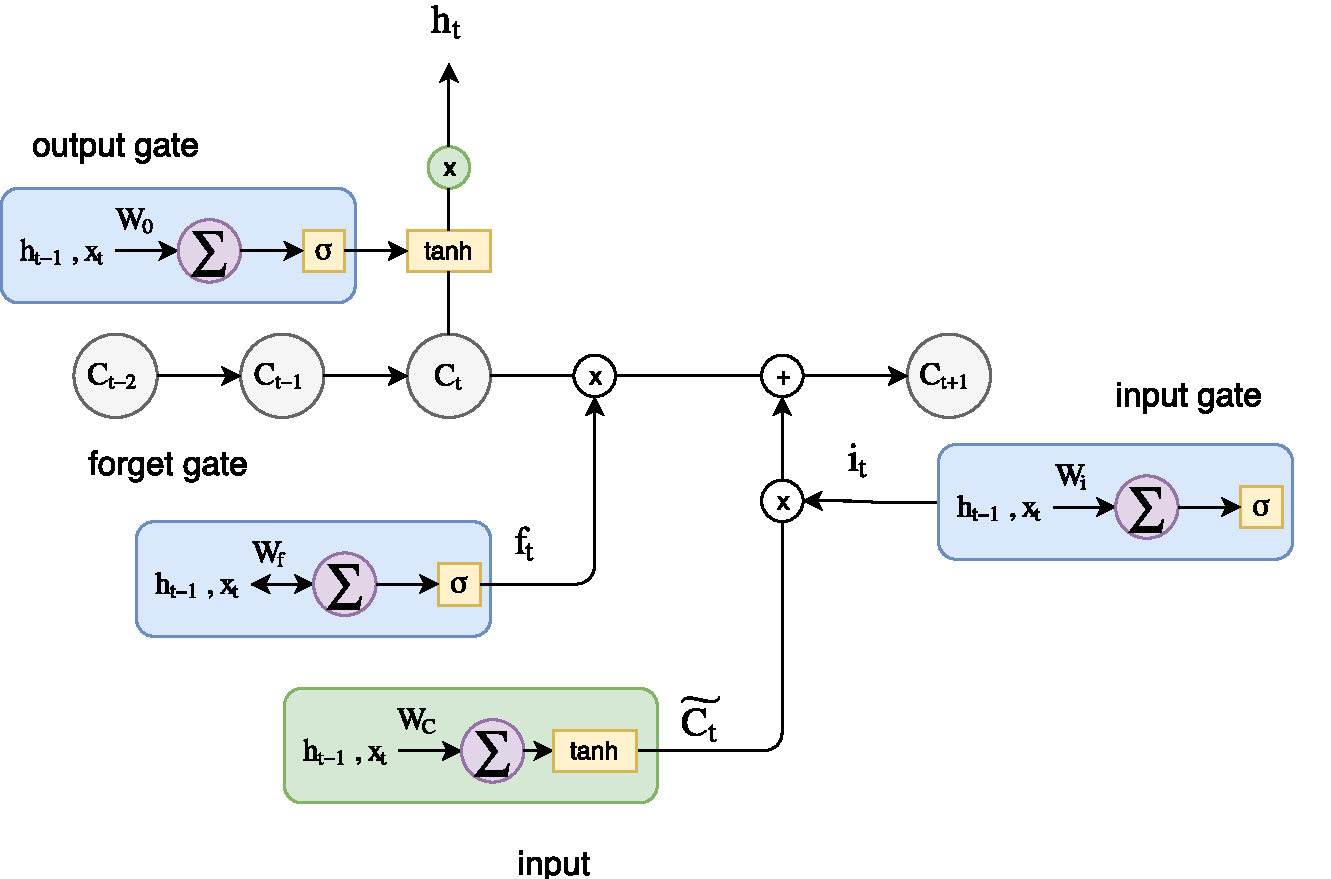
\includegraphics[width=0.9\textwidth]{Figures/LSTM}
	\caption{LSTM functionality}
	\label{LSTMcore}
\end{figure}

Having explained the LSTM functionality, the formula for computing the next time-step activity $C_{t+1}$ is the following:
\begin{equation}\label{LSTM}
C_{t+1}=f_{t}\odot C_{t}+i_{t}\odot \widetilde{C_{t}}
\end{equation}

The GRU gating approach is a simplified version of the LSTM. It actually combines all the gates into a single update:
\begin{equation}\label{GRU}
\begin{aligned}
h_{t}&=(1-z_{t})\cdot h_{t-1}+z_{t}\cdot \widetilde{h_{t}}\\
z_{t}&=\sigma(W_{z}\cdot[h_{t-1},x_{t}]) \textup{ (update gate)}\\
\widetilde{h_{t}}&=\textup{tanh}(W\cdot[r_{t}\cdot h_{t-1},x_{t}]) \textup{ (input gate)}\\
r_{t}&=\sigma(W_{r}\cdot[h_{t-1},x_{t}]) \textup{ (remember gate)}
\end{aligned}
\end{equation}